\documentclass{extreport}

\usepackage[12pt]{extsizes}
\usepackage[T2A]{fontenc}
\usepackage[utf8]{inputenc}
\usepackage[english,ukrainian]{babel}

\usepackage[a4paper, top=10mm, bottom=15mm, left=20mm, right=15mm]{geometry}
\usepackage{amsmath,amsfonts,amssymb,amsthm,mathtools}
\usepackage{listings}
\usepackage{graphicx}
\usepackage{enumitem}
\usepackage{verbatim}
\usepackage{listings}
\usepackage{xcolor}
\usepackage{textgreek}
\usepackage{diagbox}
\usepackage{pgfplots}
\pgfplotsset{compat = 1.16}

\usepackage{dsfont}

\usepackage[psdextra]{hyperref}
\hypersetup{unicode=true}
\hypersetup{
    colorlinks=true,
    linkcolor=blue,
}

\usepackage{epigraph}
\usepackage{multirow}
\usepackage{hhline}
\usepackage[normalem]{ulem}

\renewcommand{\P}{\mathbb{P}}
\newcommand{\E}{\mathbb{E}}
\newcommand{\D}{\mathbb{D}}
\newcommand{\K}{\mathbb{K}}
\newcommand{\N}{\mathbb{N}}
\newcommand{\R}{\mathbb{R}}
\newcommand{\task}[1]{\vspace{0.5em}\noindent\textbf{#1.}}

\lstdefinestyle{output_txt}{
    basicstyle=\ttfamily\footnotesize,
    breakatwhitespace=false,         
    breaklines=true,                 
    captionpos=b,                    
    keepspaces=true,                                    
    numbersep=5pt,                  
    showspaces=false,                
    showstringspaces=false,
    showtabs=false,                  
    tabsize=2
}
\definecolor{codegreen}{rgb}{0,0.6,0}
\definecolor{codegray}{rgb}{0.5,0.5,0.5}
\definecolor{codepurple}{rgb}{0.58,0,0.82}
\lstdefinestyle{python_code}{ 
    commentstyle=\color{codegreen},
    keywordstyle=\color{magenta},
    numberstyle=\tiny\color{codegray},
    stringstyle=\color{codepurple},
    basicstyle=\ttfamily\footnotesize,
    breakatwhitespace=false,         
    breaklines=true,                 
    captionpos=b,                    
    keepspaces=true,                            
    numbersep=5pt,                  
    showspaces=false,                
    showstringspaces=false,
    showtabs=false,                  
    tabsize=4
}

\setlist[enumerate]{nosep}
\graphicspath{{pics/}}
\DeclareGraphicsExtensions{.png}

\usepackage{tikz}
\makeatletter
\newcommand\mathcircled[1]{%
  \mathpalette\@mathcircled{#1}%
}
\newcommand\@mathcircled[2]{%
  \tikz[baseline=(math.base)] \node[draw,circle,inner sep=1pt] (math) {$\m@th#1#2$};%
}
\makeatother

\begin{document}
\begin{center}
    \textbf{Домашня контрольна (вона ж розрахункова, вона ж лабораторна) робота \\
    на тему <<Процесс Пуассона та елементи страхової математики>>}

    Олексій Галганов, КА-81
\end{center}

\epigraph{
    Системний дослідник повинен знати, як використовувати те, що знає; 
    розуміти, що необхідно додатково знати, чого він не знає;
    як і де дізнатися те, чого він не знає.
}{\textit{Н. Д.}}

Розглядаємо процес страхового ризику $U$, який згідно з моделлю Крамера-Лундберга має вигляд
\begin{gather}
    U(t) = u_0 + ct - \sum_{i=1}^{N(t)} X_i, \; t \geq 0
\end{gather}
де $u_0 = U(0)$ --- початковий капітал, $c$ --- сумарна величина страхових внесків за одиницю часу,
$N$ --- однорідний процесс Пуассона з інтенсивністю $\lambda > 0$, стрибки якого відбуваються в моменти настання страхових подій,
$X_i, i \in \N$ --- незалежні між собою та від $N$ однаково розподілені м.н. невід'ємні страхові виплати. Розподіл страхових виплат задано
щільністю розподілу:
\begin{gather}
    f(x) = \frac{\sin x}{2} \cdot \mathds{1}_{[0,\pi]}(x)
\end{gather}
Одразу варто обчислити функцію розподілу $X_i$ та її обернену на проміжку $[0, \pi]$, яка знадобиться для моделювання цих величин:
\begin{gather}
    F(x) = \int_0^x f(t) dt = \begin{cases}
        0, & x < 0 \\
        \frac{1}{2} \left(1 - \cos x\right), & 0 \leq x < \pi \\
        1, & x \geq \pi
    \end{cases} \\
    F^{-1}(y) =  \arccos(1-2y), \; 0 \leq y < 1 
\end{gather}
Також, обчислимо математичне сподівання $\mu = \E X$:
\begin{gather*}
    \mu = \frac{1}{2}\int_0^\pi x \sin x dx = \frac{1}{2} \left(
        - \left. x \cos x \right|_0^\pi + \int_0^\pi \cos x dx
    \right) = \frac{\pi}{2}
\end{gather*}

\textit{Let the show begin!}
\newpage

\task{Пункти 1, 2} \emph{Записати умову NPC у вигляді $c > \text{число}$.} Оскільки NPC --- це $c > \lambda \mu$, то для
двох випадків ($u_0 = 1, \lambda = 1$ та $u_0 = 10, \lambda = 5$) маємо відповідно 
$c > \frac{\pi}{2}$ та $c > \frac{5\pi}{2}$. Як і сказано, покладемо для обох випадків відповідно
$c = 2 \lambda \mu = \pi$ та $c = 1.05 \lambda \mu = 2.625 \pi$. Дуже цікаво подивитися на цей дивний світ, де за одиницю часу
вносят рівно $\pi$ умовних одиниць грошей...

\task{Пункт 3} \emph{В явному вигляді записати інтегральне рівняння для ймовірності небанкрутства $\varphi(u), u \geq 0$.} 
За теорією це рівняння має вигляд
\begin{gather}\label{main_eq}
    \varphi(u) = \varphi(0) + \frac{\lambda}{c} \int_0^u \varphi(u - y) \left(1 - F(y)\right) dy, \; u \geq 0
\end{gather}
Оскільки 
\begin{gather}\label{cdf_tail}
    1-F(y) = \begin{cases}
        1, & y < 0 \\
        \frac{1}{2} \left(1 + \cos y\right), & 0 \leq y < \pi \\
        0, & x \geq \pi
    \end{cases}
\end{gather}
то маємо таку версію інтегрального рівняння \eqref{main_eq}:
\begin{gather}
    \varphi(u) = \begin{cases}
        \varphi(0) + \frac{\lambda}{2c} \int_0^u \varphi(u - y) \left(1 + \cos y\right) dy, & 0 \leq u < \pi \\
        \varphi(0) + \frac{\lambda}{2c} \int_0^\pi \varphi(u - y) \left(1 + \cos y\right) dy, & u \geq \pi
    \end{cases}
\end{gather}

\task{Пункт 4} \emph{У максимально простому вигляді записати перетворення Лапласа $\Phi(p)$ від функції $\varphi(u)$.} Припустимо одразу, що NPC виконується,
тоді $\varphi(0) = 1 - \frac{\lambda \mu}{c}$. Після застосування перетворення Лапласа до інтегрального рівняння \eqref{main_eq} в загальному вигляді отримаємо
\begin{gather*}
    \Phi(p) = \left(1 - \frac{\lambda \mu}{c}\right) \cdot \frac{1}{p} + \frac{\lambda}{c} \cdot
    \Phi(p) \cdot \mathcal{L}\left\{1 - F(y)\right\}(p)
\end{gather*}
Знайдемо $\mathcal{L}\left\{1 - F(y)\right\}(p)$:
\begin{gather*}
    \mathcal{L}\left\{1 - F(y)\right\}(p) = \int_0^{+\infty} \left(1 - F(y)\right) e^{-py} dy = 
    \int_0^{\pi} \frac{1}{2} \left(1 + \cos y\right)e^{-py} dy = \\ =
    \frac{1}{2} \int_0^{\pi} e^{-py} dy + \frac{1}{2} \int_0^{\pi} \cos (y) e^{-py} dy \; \mathcircled{=} \\
    \int_0^{\pi} \cos (y) e^{-py} dy = \int_0^{\pi} e^{-py} d (\sin y) = \left. e^{- py} \sin y \right|_0^\pi + 
    p \int_0^{\pi} \sin (y) e^{-py} dy = \\ =
    - p \int_0^{\pi} e^{-p y} d(\cos y) = \left. -p e^{- py} \cos y \right|_0^\pi - p^2 \int_0^{\pi} \cos (y) e^{-py} dy \Rightarrow \\
    \Rightarrow (p^2 + 1) \int_0^{\pi} \cos (y) e^{-py} dy = p \left(1 + e^{-\pi p}\right) \\
    \mathcircled{=} \; \frac{1}{2} \left(
        \frac{1 - e^{-\pi p}}{p} + \frac{p \left(1 + e^{-\pi p}\right)}{p^2 + 1}
    \right) = \frac{1}{2} \cdot \frac{
        1 + 2p^2 - e^{-\pi p}
    }{
        p (p^2 + 1)
    }
\end{gather*}
Тепер можемо виразити $\Phi(p)$:
\begin{gather*}
    \Phi(p) = 
    \frac{1 - \frac{\lambda \mu}{c}}{
        p \left(1 -  \frac{\lambda}{c} \cdot \mathcal{L}\left\{1 - F(y)\right\}(p) \right)
    } = \frac{
        1 - \frac{\lambda \mu}{c}
    }{
        p - \frac{\lambda}{2c} \cdot \frac{
            1 + 2p^2 - e^{-\pi p}
        }{
            p^2 + 1
        }
    } = \\ = \left(1 - \frac{\lambda \mu}{c}\right) \cdot
    \frac{p^2 + 1}{
        p^3 + p - \frac{\lambda}{2c} \cdot
        \left(1 + 2p^2 - e^{-\pi p}\right)
    }
\end{gather*}
Для першого випадку, при $c = 2\lambda \mu$, отримаємо
\begin{gather}
    \Phi(p) = \frac{1}{2} \cdot
    \frac{p^2 + 1}{
        p^3 + p - \frac{1}{2\pi} \cdot
        \left(1 + 2p^2 - e^{-\pi p}\right)
    }
\end{gather}
Для другого, при $c = 1.05\lambda \mu$, отримаємо
\begin{gather}
    \Phi(p) = \frac{1}{21} \cdot
    \frac{p^2 + 1}{
        p^3 + p - \frac{1}{1.05 \pi} \cdot
        \left(1 + 2p^2 - e^{-\pi p}\right)
    }
\end{gather}

\task{Пункт 5} \emph{На часовому проміжку $[0, 10]$ змоделювати та побудувати на спільному рисунку графіки $5$ траєкторій процесу $U$.}
\begin{center}
    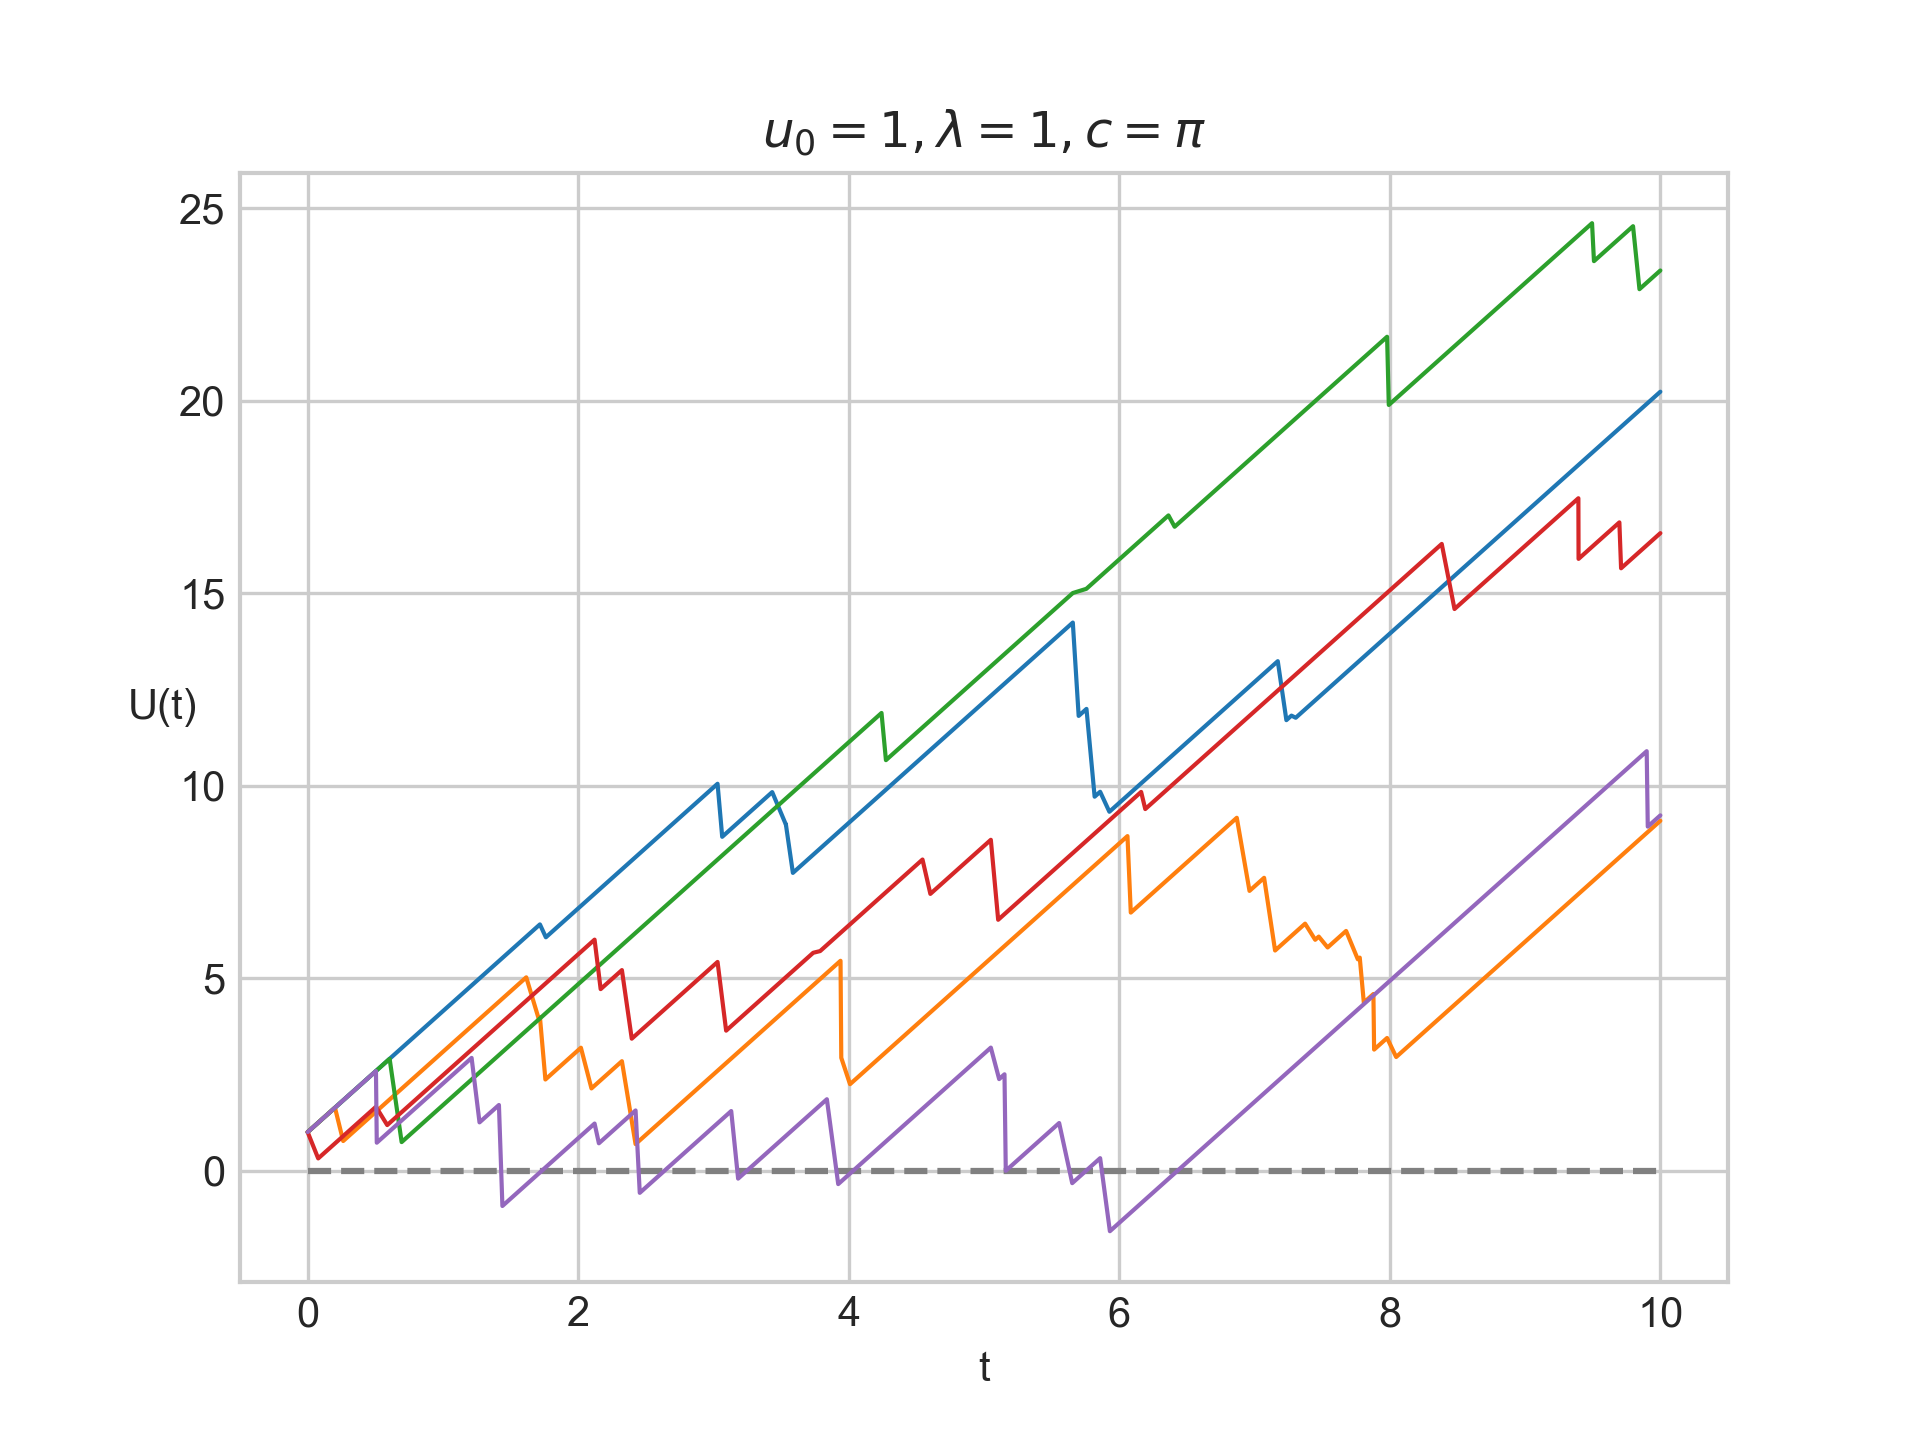
\includegraphics[scale=0.95]{trajectories_1.png} \\
    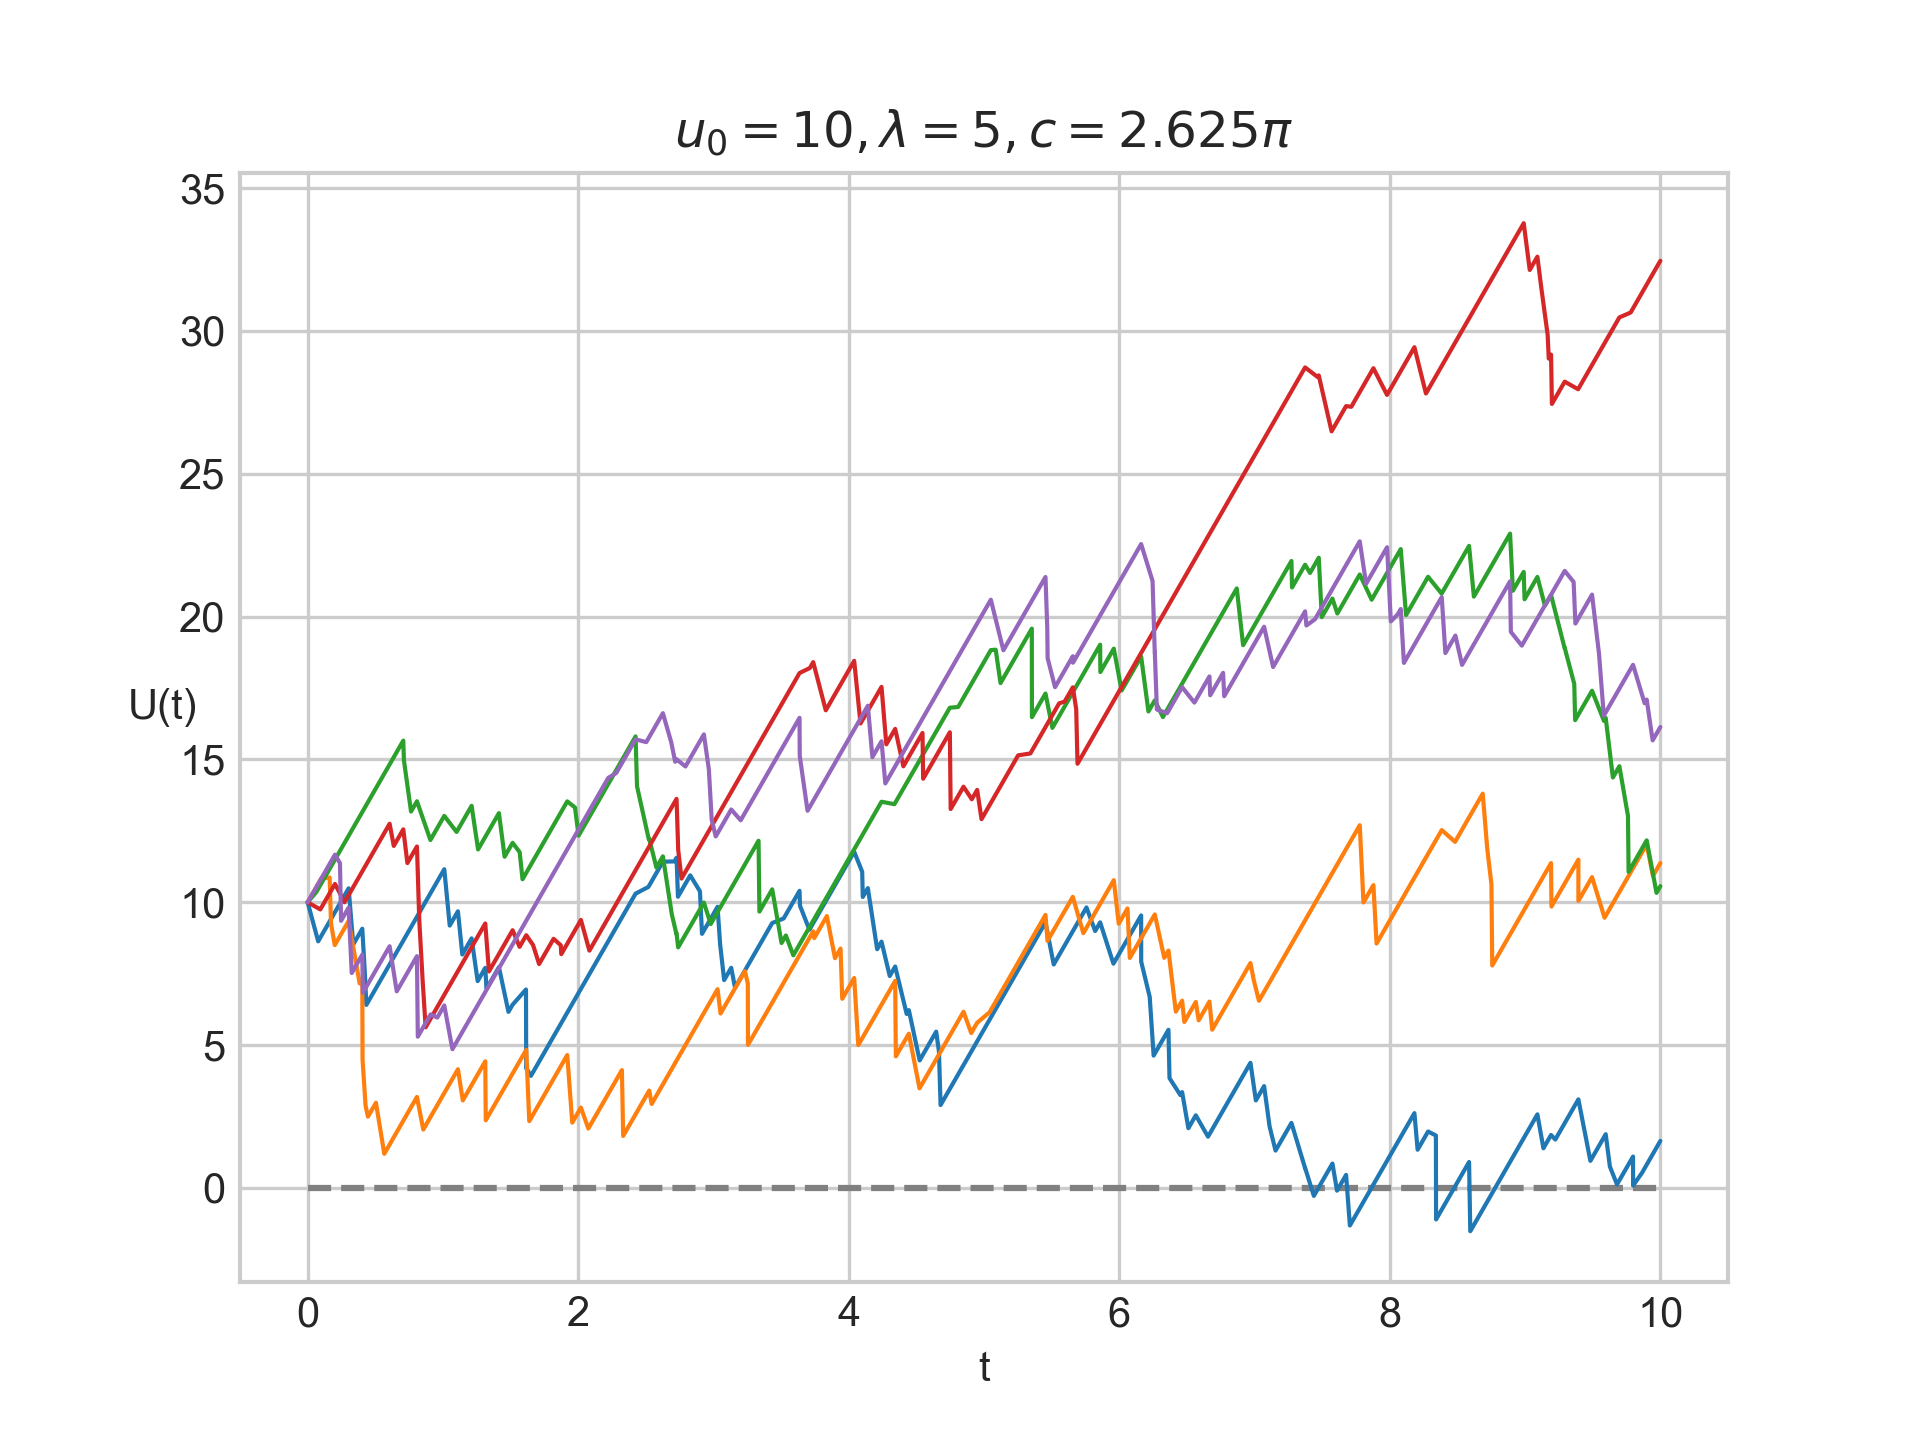
\includegraphics[scale=0.95]{trajectories_2.png}
\end{center}
\task{Пункт 6} \emph{Оцінити ймовірність банкрутства за допомогою грубого методу Монте-Карло: для цього на проміжку $[0, 1000]$
змоделювати 1000 траєкторій процесу $U$ й обчислити частку тих, що банкрутують протягом цього проміжку.}
Можна також згадати Ірину Юріївну та довірчий інтервал для ймовірності появи події, межі якого для великої кількості випробувань визначаються з 
\begin{gather*}
    p_{1, 2} = p^* \pm t_{\gamma} \sqrt{\frac{p^* \left(1 - p^*\right)}{n}}
\end{gather*}
де $t_{\gamma}$ --- значення оберненої функції Лапласа в точці $\gamma / 2$ для рівня надійності $\gamma$.

Отже, для першого випадку отримаємо оцінку ймовірності банкрутства $p^* = 0.317$ з 95\% довірчим інтервалом $(0.288, 0.346)$,
а для другого --- $p^* = 0.579$ та $(0.5484, 0.61)$.

\task{Пункт 7} \emph{Оцінити ймовірність банкрутства за допомогою більш точного методу Монте-Карло: для цього спочатку записати функцію розподілу
модифікованої величини $\tilde{X}$, а потім змоделювати геометрично розподілену кількість незалежних копій цієї величини.} За теорією,
функція розподілу $\tilde{X}$ має вигляд
\begin{gather}
    F_{\tilde{X}}(x) = \frac{1}{\E X} \int_0^x \left(1 - F_X(t)\right) dt
\end{gather}
Скориставшись виразом для $1 - F_X(t)$ з \eqref{cdf_tail}, отримаємо 
\begin{gather}
    F_{\tilde{X}}(x) = \begin{cases}
        0, & x < 0 \\
        \frac{2}{\pi} \int_0^x \frac{1}{2}\left(1 + \cos t\right) dt = \frac{1}{\pi} \left(x + \sin x\right), & 0 \leq x < \pi \\
        \frac{2}{\pi} \int_0^{\pi} \frac{1}{2}\left(1 + \cos t\right) dt = 1, & x \geq \pi 
    \end{cases}
\end{gather}
Обернену до функцію розподілу в цьому випадку вже неможливо обчислити в явному вигляді, тому
для моделювання цих величин будемо використовувати чисельно знайдену обернену функцію.

Згідно з модифікованим методом Монте-Карло, ймовірність банкрутства при початковому капіталі $u$ обчислюється з формули
\begin{gather*}
    \psi(u) = 1 - \varphi(u) = 1 - \P\left\{
        \tilde{X}_1 + \tilde{X}_2 + \dots + \tilde{X}_G \leq u
    \right\} = \P\left\{
        \tilde{X}_1 + \tilde{X}_2 + \dots + \tilde{X}_G > u
    \right\}
\end{gather*}
де $G \sim \mathrm{Geom}\left(1 - \frac{\lambda \mu}{c}\right)$. Отже, для оцінки ймовірності банкрутства змоделюємо 1000 значень $G$,
після чого для кожного значення треба реалізувати відповідну кількість значень незалежних $\tilde{X}_i$ та обчислити, 
скільки разів їх сума перевищить значення початкового капіталу $u_0$.
Для першого випадку отримаємо оцінку ймовірності банкрутства $p^* = 0.325$ з 95\% довірчим інтервалом $(0.296, 0.354)$,
а для другого --- $p^* = 0.583$ та $(0.5524, 0.6136)$.

\task{Пункт 8} \emph{Оцінити ймовірність банкрутства за допомогою чисельного знаходження оберненого перетворення Лапласа.}
Можна навіть побудувати графіки залежності ймовірності банкрутства $\psi(u)$ від початкового капіталу $u$. Для першого випадку 
$\psi(u_0) = \psi(1) \approx 0.32745$:
\begin{center}
    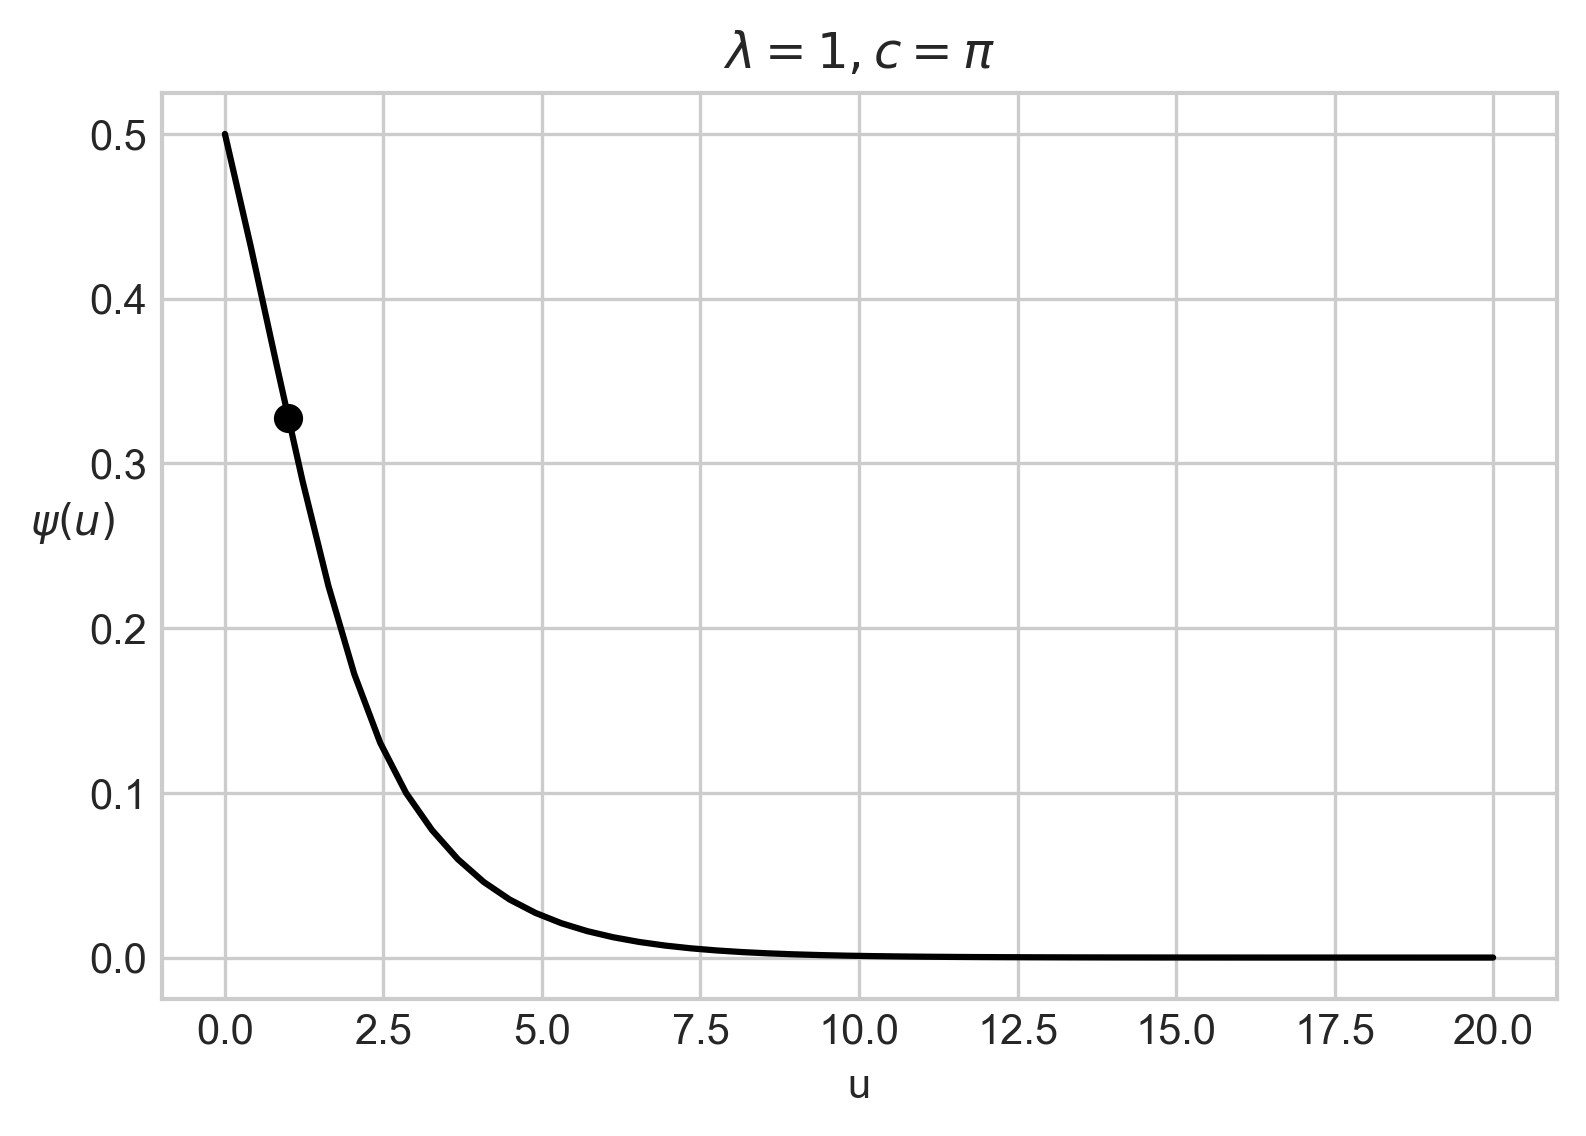
\includegraphics[scale=0.7]{psi_1.png}
\end{center}
Для другого випадку $\psi(u_0) = \psi(10) \approx 0.57576$:
\begin{center}
    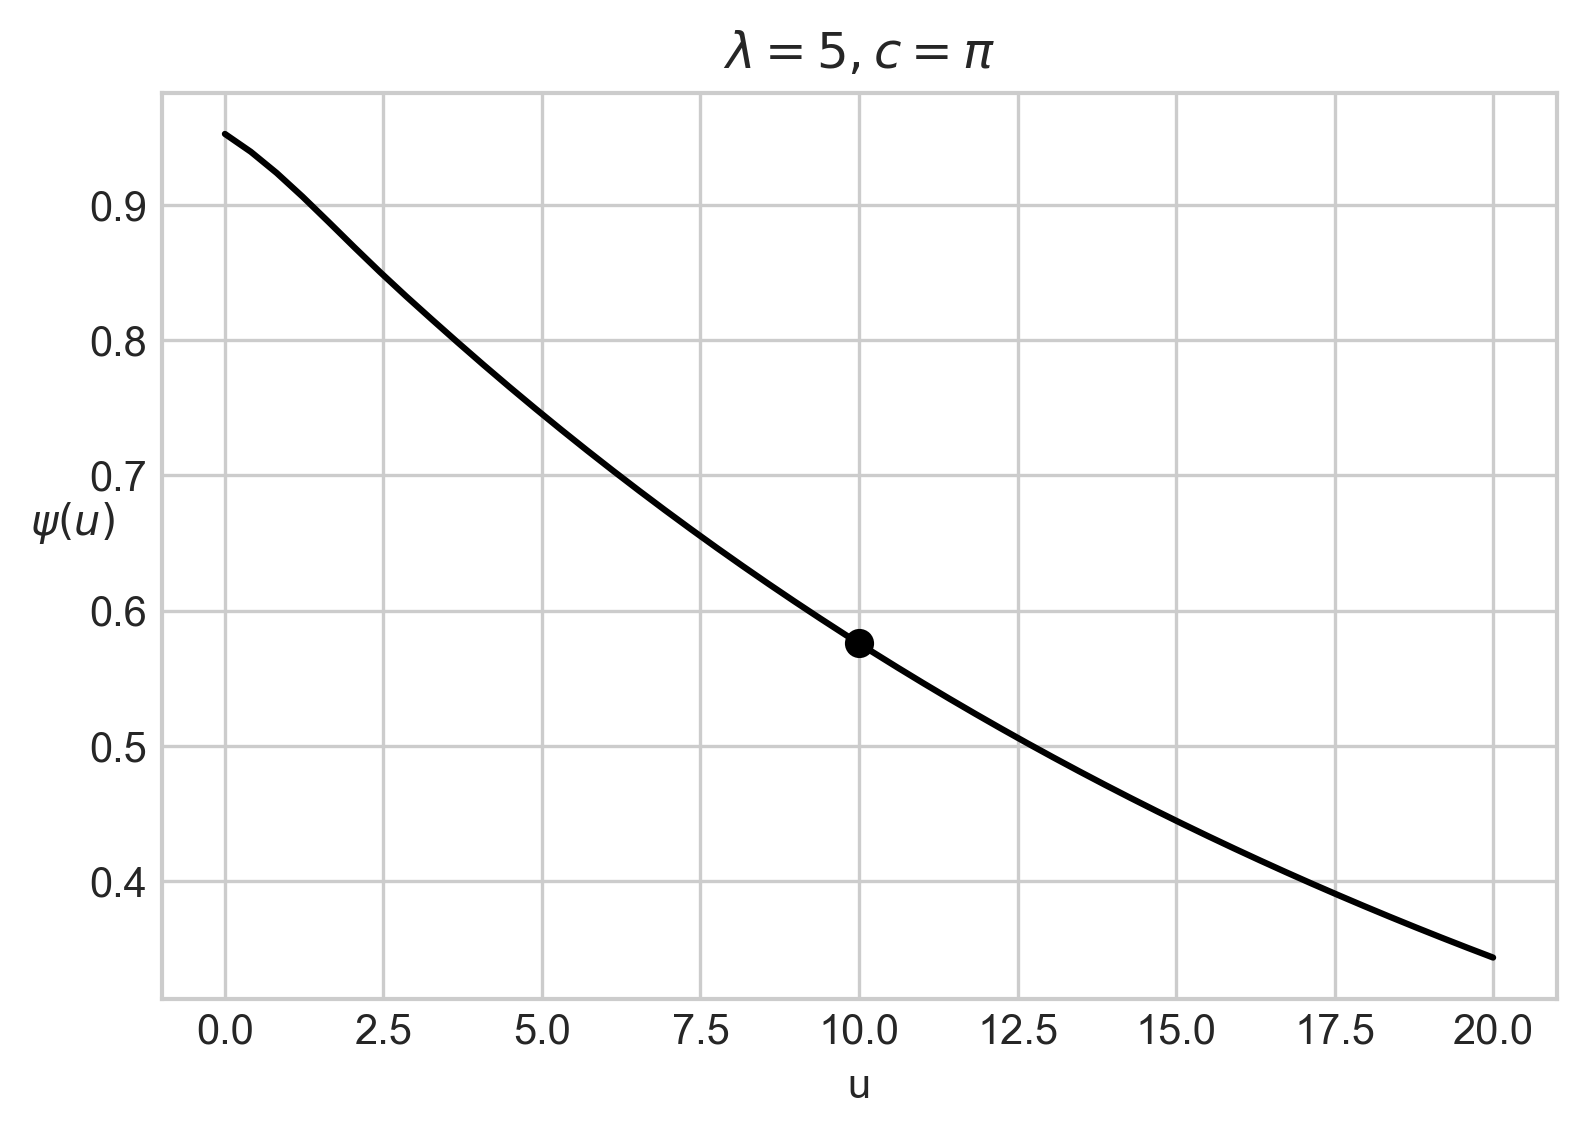
\includegraphics[scale=0.7]{psi_2.png}
\end{center}

\task{Висновки} Зведемо отримані результати до таблиці:
\begin{center}
    \begin{tabular}{|c|c|c|c|c|}
        \hline
        \multicolumn{2}{|c}{\textbf{грубий ММК}} & \multicolumn{2}{|c|}{\textbf{більш точний ММК}} & \multirow{2}{*}{\textbf{обернене перетворення Лапласа}} \\
        \cline{1-4}
        оцінка & інтервал & оцінка & інтервал & \\
        % \hhline{|=|=|=|=|=|}
        \hline
        \multicolumn{5}{|c|}{\emph{випадок 1: $u_0 = 1, \lambda = 1, c = 2 \lambda \mu$}} \\
        \hline
        $0.317$ & $(0.288, 0.346)$ & $0.325$ & $(0.296, 0.354)$ & $0.32745$ \\ 
        % \hhline{|=|=|=|=|=|}
        \hline
        \multicolumn{5}{|c|}{\emph{випадок 2: $u_0 = 10, \lambda = 5, c = 1.05 \lambda \mu$}} \\
        \hline
        $0.579$ & $(0.5484, 0.61)$ & $0.583$ & $(0.5524, 0.6136)$ & $0.57576$ \\ 
        \hline
    \end{tabular}
\end{center}
Отже, \sout{в ході виконання лабораторної роботи було виконано лабораторну роботу} можна побачити,
що для обох випадків оцінки обома методами Монте-Карло не надто відрізняються, але оцінки більш точним методом більші,
ніж грубим (і так було не один раз при моделюванні) --- це можна пояснити тим, що грубий метод не враховує настання банкрутства на 
інтервалі $\left(1000, +\infty\right)$. Оцінку ймовірності банкрутства за допомогою оберненого перетворення Лапласа можна вважати найбільш наближеною до реальності,
оскільки в цьому випадку з обчислень виключається випадковість, а чисельні методи можуть дати значення з якою завгодно точністю.
Але в той же час, ці значення не надто відрізняються від оцінок ММК, тому усі три розглянуті методи оцінки ймовірності банкрутства мають право на життя:
\begin{enumerate}
    \item[--] перевагою грубого ММК є простота реалізації, оскільки немає потреби в додаткових аналітичних обчисленнях, але недоліком ---
    неврахування можливого банкрутства за межею відрізку часу, що розглядається;
    \item[--] перевагою оберненого перетворення Лапласа є висока точність та можливість побудувати як завгодно точно графіки $\varphi(u)$ та $\psi(u)$,
    але для застосування цього методу треба мати явний вигляд $\Phi(p)$ та вміти обчислювати чисельно обернене перетворення;
    \item[--] більш точний ММК є таким собі компромісом між двома іншими, оскільки додатково обчислювати потрібно лише функцію розподілу $\tilde{X}$,
    причому можна покластися і на чисельне інтегрування, а точність обчислення можна покращувати, посилаючись за ЗВЧ та генеруючи більше значень $G$: 
    наприклад, для другого випадку при моделюванні 10000 значень отримаємо оцінку $0.5718$ з довірчим інтервалом $(0.5621, 0.5815)$,
    а для 100000 --- $0.57856$ та $(0.5755, 0.5816)$ відповідно.
\end{enumerate}
В той же час, якщо уявити, що відомо лише емпіричний розподіл виплат, то застосовність двох останніх методів буде від питанням. 
Для більш точного ММК, оскільки розподіли $\tilde{X}$
та $G$ (через наближене значення $\mu$) також будуть деяким наближенням до реальних розподілів цих величин, то точність отриманих оцінок може погіршитись
через накопичення різних похибок. Щодо обчислення оберненого перетворення Лапласа, в цілому складно сказати,
як використання емпіричної функції розподілу вплине на оцінку цим методом: перетворення такої ступінчастої функції матиме досить складний вид
(зважена сума образів зсунутої функції Хевісайда), що також може вплинути на чисельне обчислення оберненого перетворення.
\end{document}